\subsection{Occam's Razor and the Pareto Front \quad / \quad \textthai{มีดโกนของออคแคมและ Pareto Front}}
\begin{paracol}{2}
A fundamental principle in physics is **Occam's Razor**\index{Occam's Razor@มีดโกนของออคแคม (Occam's Razor)}: the simplest explanation is usually the correct one. In the context of Symbolic Regression, this principle is quantified as the trade-off between \textbf{Accuracy} (Mean Squared Error) and \textbf{Mathematical Complexity} (the number of operators, constants, and variables in the expression tree).

Technically, we seek the \textbf{Pareto Front}\index{Pareto Front@Pareto Front (Pareto Front)}—a set of non-dominated solutions. As shown in Figure \ref{fig:ch8_pareto}, the Pareto Front represents the optimal balance. Each point on this curve is an equation that cannot be made simpler without losing accuracy, nor made more accurate without becoming significantly more complex.

For a physicist, the "truth" often lies at the \textbf{Elbow}\index{Elbow Point@จุดข้อศอก (Elbow Point)} of this curve—the point where complexity is minimal but accuracy is exceptionally high. This is precisely how AI identifies laws like $F=ma$ or $E=mc^2$ from noisy experimental data.

\begin{figure}[ht]
    \centering
    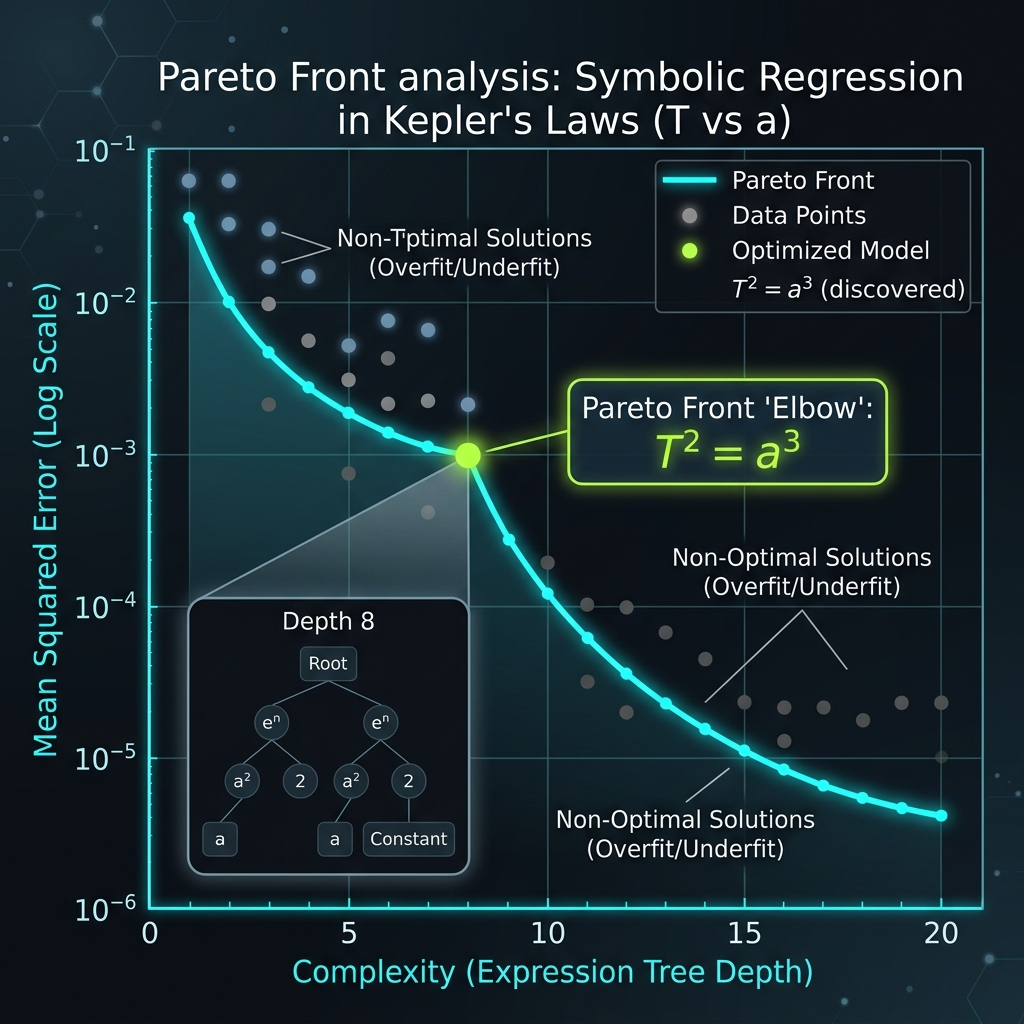
\includegraphics[width=0.85\textwidth]{assets/ch8_results.png}
    \caption{Pareto Front analysis for Kepler's Law discovery. The highlighted point represents the discovery of $T^2 = a^3$ where complexity and error are optimally balanced.}
    \label{fig:ch8_pareto}
\end{figure}

\switchcolumn

\begin{thai}
หลักการพื้นฐานในทางฟิสิกส์คือ **มีดโกนของออคแคม (Occam's Razor)** ซึ่งกล่าวว่าคำอธิบายที่เรียบง่ายที่สุดมักจะเป็นคำอธิบายที่ถูกต้อง ในบริบทของการถดถอยเชิงสัญลักษณ์ หลักการนี้จะถูกวัดด้วยปริมาณผ่านการแลกเปลี่ยนระหว่าง \textbf{ความแม่นยำ (Accuracy)} และ \textbf{ความซับซ้อนทางคณิตศาสตร์ (Mathematical Complexity)} (จำนวนตัวดำเนินการ ค่าคงที่ และตัวแปรใน Expression Tree)

ในทางเทคนิค เรากำลังมองหา **Pareto Front** ซึ่งเป็นชุดของคำตอบที่ไม่มีตัวเลือกอื่นครอบงำ (Non-dominated solutions) ดังที่แสดงในรูปที่ \ref{fig:ch8_pareto} เส้นโค้ง Pareto Front แสดงถึงความสมดุลที่เหมาะสมที่สุด แต่ละจุดบนเส้นโค้งนี้คือสมการที่ไม่สามารถทำให้เรียบง่ายกว่านี้โดยไม่สูญเสียความแม่นยำ และไม่สามารถทำให้แม่นยำขึ้นได้โดยไม่เพิ่มความซับซ้อนอย่างมหาศาล

สำหรับนักฟิสิกส์ "ความจริง" มักตั้งอยู่ที่ **จุดข้อศอก (Elbow Point)** ของเส้นโค้งนี้ ซึ่งเป็นจุดที่ความซับซ้อนน้อยที่สุดแต่มีความแม่นยำสูงเป็นพิเศษ นี่คือวิธีที่ AI ระบุกฎต่างๆ เช่น $F=ma$ หรือ $E=mc^2$ จากข้อมูลการทดลองที่มีสัญญาณรบกวน
\end{thai}
\end{paracol}
